\chapter{Monads}
\section{Overview}


\subsection{History}
In May 1996, the Haskell report 1.3 is published ,in this version , monadic IO as well as do-notation made its first appearance.[A History of Haskell:Being Lazy With Class] \\

In April 1997,the list comprehension is generalised into monad in the Haskell report 1.4.[A History of Haskell:Being Lazy With Class]\\ 

Nowadays ,a monad has become a de-facto pattern for Haskell programmer who wants to monad and write computation with side effect,and this pattern is explicitly supported by Haskell.\\


Pure languages are easier to reason about and may benefit from lazy
evaluation, while impure languages offer efficiency benefits and sometimes make possible a more compact mode of expression.[Monads for functional programming]



\subsection{Side effect}
In imperative language like C/C++ , it is often the case that it access the variable outside the function,eg. the error flag.In Java, the keyword \textbf{synchronized} is used to acquire look to the share resource,most of time,they are the resource from out side word.\\

Imperative language are unrestricted to side effect,which makes it hard to write function that allows parallelism .On the other hand,Haskell restricts side effects with a static type system; it uses the concept of monads to do "stateful" and IO computations.[Imperative Functional Programming]\\

Another approach to introducing effects in a purely functional language
is to make the use of effects explicit in the type system. Several methods
have been proposed, but the most elegant and widely used is the concept
of a monad.[Imperative Functional Programming]  Monads in Haskel have been used to model IO,state,logger,error as well as List.



\section{Introduction to Monad}
In Haskell,monad is used an abstract data type constructor to represent multiple kinds of computation such as a computation that will do IO action,or a computation that has state.Those computations are in-pure because that manipulate the outside world.In Haskell.Mathematically, monads are governed by set of laws that should hold for the monadic operations [A Gentle Introduction to Haskell, Version 98]. There are two basic law in monads ,they are bind return .The Monad class is defined as follow:
\begin{hcode}
class Monad m where
  (>>=) :: m a -> (a -> m b) -> m b
  (>>) :: m a -> m b -> m b
  return :: a -> m a
  fail :: String -> m a
\end{hcode}

The return function can inject a value into monadic type.
The bind function can combine two monadic function, one should be of type \textbf{m a} and another should be of type \textbf{a -$>$ m b} .

Beside this two function,Haskell also provide other monadic operator which all derive from \textbf{return} and \textbf{bind},they are:
\begin{hexample}
liftM :: (Monad m) => (a1 -> r) -> m a1 -> m r
liftM2  :: (Monad m) => (a1 -> a2 -> r) -> m a1 -> m a2 -> m r
ap :: (Monad m) => m (a -> b) -> m a -> m b
(=<<) :: (Monad m) => (a -> m b) -> m a -> m b
\$ ::(m a -> m b) -> m a -> m b 
\end{hexample}

These monadic operation is define using the bind and return.For example ,liftM is defined by bind and return like 
\begin{hcode}
liftM f m1              = do { x1 <- m1; return (f x1) }
\end{hcode}
Therefore,when defining a monad,only bind and return need to be specified.

\subsubsection{Monad Laws}
For all monad instance ,beside define three monadic operator ,they must apply three compulsory monad laws:
\begin{hcode}
"Left identity": return a >>= f  ≡  f a
"Right identity": m >>= return  ≡  m
"Associativity": (m >>= f) >>= g  ≡  m >>= (\x -> f x >>= g)
\end{hcode}

In monad instance ,these monad laws will become a restriction of the operation when combining monadic function using monadic operation,these restriction will be discussed in following sections.


\subsubsection{Monadic Function}
A monadic function is function that produce , however,monadic function like \textbf{putStr :: String -$>$ IO ()} can not be combined using \\ \textbf{(.) :: (b -$>$ c) -$>$ (a -$>$ b) -$>$ a -$>$ c}.Monadic class constructor has tag 



\section{IO Monad}
Haskell use IO monad to limit the IO sequence.Monadic operation are used to represent IO processing pipeline.\\

Haskell I/O has always been a source of confusion and surprises for new Haskellers.

Normally, the first thing to lean a new language to to print something on the screen,but it is not the case in Haskell.The first thing I do in Haskell is to write a quick sort algorithm which is a classic program to show the powerful Haskell list comprehension feature that brings the most elegant solution of quick sort compared to most of other language.On the other hand,its not that straight forward to build an IO system upon it inside language that emphasized purity.



It probably not the best monad for beginner to learn as it dost not provide escape function.The IO moand is implemented as part of language in \textbf{Base.GHC},thus the logic of monad operator is not exposed to outside world.

\begin{hcode}
unsafePerformIO :: IO a -> a
\end{hcode}

The above shows the code of an escape function which will break the purity of Haskell IO system.This is the "back door" into the IO monad, allowing IO computation to be performed at any time. For this to be safe, the IO computation should be free of side effects and independent of its environment.[ haskell io document]


As we can guess from the nature of Haskell,IO monad is introduced to guarantee to following factor,

\begin{itemize}
\item The sequence of IO actions perform in a lazy Haskell context.
\item perform IO as an function rather than a function or and command in functional programming context.
\item combine IO,distinguish computation that with IO actions with the one without.
\item  file buffering , open and close file in a correct manner.
\end{itemize}


The code below shows combination of monad using bind operator.
\begin{hcode}
ioAction 
  =putStrLn "What is your name ?"
	 >>= (_-> getLine >>= 
		(\x -> putStrLn ("welcome" ++ x) ))
\end{hcode}


\section{State Monad}
The basic idea of a state monad is to allow us to represent functions which interact with local state variables (which are just called local variables in most languages), or global state variables (usually called global variables). Essentially, they allow us to simulate some aspects of imperative programming in a purely functional setting.\\

An alternate solution is that we can pass the initial state into each function and return the state together with the result,with may looks like,
\begin{hcode}
add :: State -> Input -> (State ,Output)
-- implement

subtract :: State -> Input -> (State,Output)
\end{hcode}


To make it possible to composite computation with state we could rewrite all computation with follow.

\begin{hcode}
add :: (Input,State) -> (Output,State)
-- implementation 
subtract :: (Input,State) -> (Output,State)
combine = add.subtract 
\end{hcode}

However,its tedious to write all the function with computation this way.The state monad provides a way to encapsulate the state logic into a monad without explicitly specify a State type as input and output.Like IO, the computations with state  are tagged with the type constructor \textbf{State} indicating this is a state monadic function.Most importantly, the monad law and state monad implementation guarantee the follow fact of a computation with state , they are

\begin{itemize}
\item It possible to construct a new state monadic function without initial state.
\item when combine two state,from the nature of state transformation ,the change of state of  the second function is always after the first function.
\item For a computation with state,we need to need the both the result of computation as well as the final state as an output of the computation.
\end{itemize}

\begin{figure}[H]
  \centering
	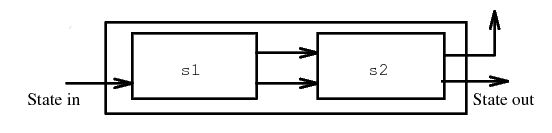
\includegraphics[width=0.80\textwidth]{pic/c3/state_monad.png}
	\caption{Combining Two "Stateful" Monadic Functions}
\end{figure}


\section{List Comprehension and List Monad}
\subsection{List Comprehension}
Haskell added syntax sugar to allow programmer to write code in a more readable manner.The list comprehension allow us to write a list using mathematics favour.

A Fibonacci series can be written as follow,
\begin{hcode}
fibs :: [Int]
fibs = 0 :1 : [ a + b | (a, b) <- zip fibs (tail fibs)]
\end{hcode}

If we view if as a mathematical expression,we can easily figure out it means $ \lbrace  0,1 ,(0+1),(1+1),(1+2),(2+3),(3+5),... \rbrace $, which will generate a Fibonacci series.In addition,it is also an example of how useful of lazy evaluation in Haskell.

\subsection{List Monad}
We can view a list as monad.In list comprehension ,we have the \textbf{$<$-} operator which we can view it as $\in$,which has a mathematical $ in$  semantic.\\

Alternatively , we can view list as an monad.
\begin{hcode}
instance  Monad []  where
  m >>= k  = concat (map k m)
  return x = [x]
\end{hcode}

The code above shows the definition of monad,the type construct is the list notation [],and the bind operator means that applying and monadic computation to a given list which is also a monadic data type. Equally,the list monad satisfy the three monad law ,namely ,left identity,right identity and associativity.\\

\begin{figure}[H]
  \centering
	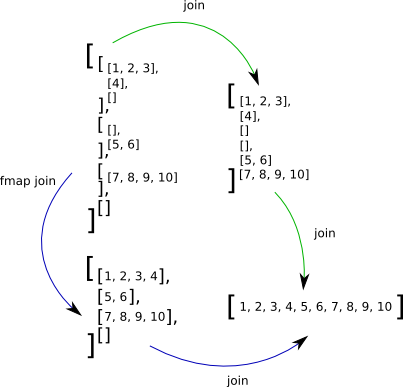
\includegraphics[width=0.60\textwidth]{pic/c3/list_monad.png}
	\caption{The First Monad Law illustration}
\end{figure} [Haskell/Category theory]



\section{Do Notation }
The do notation is a syntax sugar to write monadic operation especially bind in a imperative way ,to be more specified,only monadic function with the same return type can write together.An IO action that return \textbf{IO ()} can not put with and state monadic function that return \textbf{State s a}.

To write a get line and put line logic using bind, the sequence of IO is guaranteed by monad laws.
\begin{hcode}
 getLine >>= (\x -> putStrLn x)
\end{hcode}


Following code shows that the same functionalities are written using do-notation,which shows a strong similarity to a imperative language.
\begin{hcode}
do line <- getLine 
   putStrLn line
\end{hcode}

The \textbf{$<$-} notation in this context means unwrap the content in the monad and put it in to a variable,for example ,a monadic function returns \textbf{IO String} ,the \textbf{$<$-} notation means unwraping the content of type String from IO container.



\section{Error Monad}
The error monad can models a computation which may fail or throw exception.The construct or a error monad is \textbf{Either a b} where a represent the type of error message and b represents the normal return value.

A left value will be returned if a computation or a combination of a computation fail whereas a right will value will be returned if succeed.The code below shows the bind strategy.

\begin{hcode}
instance Monad (Either a) where
    return = Right
    x >>= f = case x of
        Left _ -> x
        Right r -> f r
\end{hcode}

From the above implementation ,we knows that for a computation x and f ,if the previous computation ,namely x has error,the second computation f will be abandoned,thus and error of x will be return.The first computation will be attempted only when the first computation succeed,the result of the first computation will be extracted from the right value and applied from the second computation.
Finally ,we can know that, for a composition of computation which may fail,the earliest failure message will be recorded.


\section{Other Monads}
Other monads includes Maybe Monad ,Reader Monad,Writer Monads , are designed to model a certain type of computation.

The Maybe monad is similar to the Error,though its just a simplified version that can not return any useful error message.\\

Reader Monad are designed to model computation that read values from a shared environment.In fact,for computations that read values from outside word,it is possible that we pass the environment variable as the parameter to functions.But it would be simplified if we use the reader monad.
The bind monad operation,which we can guess that will allow to computation to access that shared environment.\\

Equally,the Writer Monad are designed module computation that write to a shared configuration.As we can guess,the bind operator all both computation to write into the environment.


